\documentclass[a4paper,10pt]{article}

\usepackage[english]{babel}
\usepackage{multirow}
\usepackage[utf8]{inputenc}
\usepackage{a4wide}
\usepackage{longtable}
\usepackage{listings}
\usepackage{hyperref}
\usepackage{enumitem}

\usepackage{graphicx}

\usepackage{amssymb}
\usepackage{amsmath}
\usepackage{amsthm}


%opening
\title{Resolución de ecuación 1d de calor por diferencias finitas \\ en máquina sencilla
\\
Diseño de Sistemas con FPGAs - UBA}

\date{1er Cuatrimestre 2016 }

\addtolength{\topmargin}{-3cm}
\addtolength{\textheight}{4cm}

\addtolength{\oddsidemargin}{-1.5cm}
\addtolength{\textwidth}{3cm}

\begin{document}
\lstset{tabsize=2, language=C}

\maketitle

% \section*{Generalidades}

Planteo del problema: se obtendrá el perfil de temperaturas en estado estacionario de una barra de metal. Para ello se resolverá la ecuación de calor undimensional en estado estacionario, bajo apropiadas condiciones de borde.
Sea $u: \rm I\!R \to \rm I\!R $ el campo escalar de temperaturas [$^{\circ}C$].  Sea x, $x_0 \leq x \leq x_n$,  la variable independiente que representa la dimensión espacial [cm]. D la conductividad térmica del material. Resolver $\frac{\partial }{\partial x} \left( D \frac{\partial u}{\partial x} \right) = 0$. Con condiciones de borde $u(x=x_0)=u_0$ y $u(x=x_n)=u_n$. $u_0=100, u_n=0, x_0=0, x_n=150$.

% Condiciones iniciales u(x=x_0)=100, u(x=x_n)=0. u_0=100, u_n=0, x_0=1, x_n=100.

Probar que la solución analítica a este problema es la recta que pasa por los puntos $(x_0,u_0)$ y $(x_n,u_n)$ independientemente de la conductividad térmica del material.

La solución a esta ecuación simple se realiza de forma numérica, por el método de las diferencias finitas.

El esquema numérico generado es el siguiente: $r \ u_{i+1} - 2 \ r \ u_i + r \ u_{i-1} = 0$ donde r = $\frac{D}{2 \ dx}$

Al partir del cual se construye el sistema de ecuaciones:

\begin{equation*}
  \left(
  \begin{smallmatrix}
  1 & 0 & 0 & 0 & 0 & 0 & 0 & 0 & 0 & 0 & 0 & 0 & 0 & 0 & 0 & 0 \\
  r & -2r & r & 0 & 0 & 0 & 0 & 0 & 0 & 0 & 0 & 0 & 0 & 0 & 0 & 0 \\
  0 & r & -2r & r & 0 & 0 & 0 & 0 & 0 & 0 & 0 & 0 & 0 & 0 & 0 & 0 \\
  0 & 0 & r & -2r & r & 0 & 0 & 0 & 0 & 0 & 0 & 0 & 0 & 0 & 0 & 0 \\
  0 & 0 & 0 & r & -2r & r & 0 & 0 & 0 & 0 & 0 & 0 & 0 & 0 & 0 & 0 \\
  0 & 0 & 0 & 0 & r & -2r & r & 0 & 0 & 0 & 0 & 0 & 0 & 0 & 0 & 0 \\
  0 & 0 & 0 & 0 & 0 & r & -2r & r & 0 & 0 & 0 & 0 & 0 & 0 & 0 & 0 \\
  0 & 0 & 0 & 0 & 0 & 0 & r & -2r & r & 0 & 0 & 0 & 0 & 0 & 0 & 0 \\
  0 & 0 & 0 & 0 & 0 & 0 & 0 & r & -2r & r & 0 & 0 & 0 & 0 & 0 & 0 \\
  0 & 0 & 0 & 0 & 0 & 0 & 0 & 0 & r & -2r & r & 0 & 0 & 0 & 0 & 0 \\
  0 & 0 & 0 & 0 & 0 & 0 & 0 & 0 & 0 & r & -2r & r & 0 & 0 & 0 & 0 \\
  0 & 0 & 0 & 0 & 0 & 0 & 0 & 0 & 0 & 0 & r & -2r & r & 0 & 0 & 0 \\
  0 & 0 & 0 & 0 & 0 & 0 & 0 & 0 & 0 & 0 & 0 & r & -2r & r & 0 & 0 \\
  0 & 0 & 0 & 0 & 0 & 0 & 0 & 0 & 0 & 0 & 0 & 0 & r & -2r & r & 0 \\
  0 & 0 & 0 & 0 & 0 & 0 & 0 & 0 & 0 & 0 & 0 & 0 & 0 & r & -2r & r \\
  0 & 0 & 0 & 0 & 0 & 0 & 0 & 0 & 0 & 0 & 0 & 0 & 0 & 0 & 0 & 1 \\
  \end{smallmatrix} 
  \right)
  \left(
  \begin{smallmatrix}
  u(0) \\
  u(1) \\
  u(2) \\
  u(3) \\
  u(4) \\
  u(5) \\
  u(6) \\
  u(7) \\
  u(8) \\
  u(9) \\
  u(10) \\
  u(11) \\
  u(12) \\
  u(13) \\
  u(14) \\
  u(15) \\
  \end{smallmatrix} 
  \right)
=
  \left(
  \begin{smallmatrix}
  u_0 \\
  0 \\
  0 \\
  0 \\
  0 \\
  0 \\
  0 \\
  0 \\
  0 \\
  0 \\
  0 \\
  0 \\
  0 \\
  0 \\
  0 \\
  u_n \\
  \end{smallmatrix} 
  \right)

\end{equation*}

Suponiendo r=0.5 para satisfacer la condición de estabilidad, y usando el método para resolución de sistemas de ecuaciones lineales de Jacobi se obtuvo el siguiente código matlab:

\begin{lstlisting}
  clear all;
  % Inicializo el vector de temperaturas
  M = 16; 
  u_prima(1) = 32767;
  u_prima(2:M) = 0;

  % It. principal
  N = 150;
  for( k = 1 : N )
    % Sub It.
    for( i = 2 : M - 1 )
      u_prima(i) = ( u_prima(i+1) + u_prima(i-1) ) / 2;
    end 
  end 
  plot(u_prima);
\end{lstlisting}

El código ensamblador asociado, que envía los datos generados a través de la UART de la máquina sencilla se adjunta a este documento.

Debido a que este algoritmo necesita de números reales para funcionar, y que la máquina sencilla implementada no tiene este tipo de representación se optó por lo siguiente: $u'(x) = u(x) * 327.67$. En el caso de la condición de Diriclet del extremo izquierdo, $u'_0$=32767. De modo que una vez calculados los u'(x), usando la relacción anterior, se pueden obtener los valores deseados. Si bien esta alternativa pierde precisión es suficientemente buena para resolver el problema que se plantea.

El peril de temperaturas generados es:

\begin{minipage}[h!bt]
    \centering
    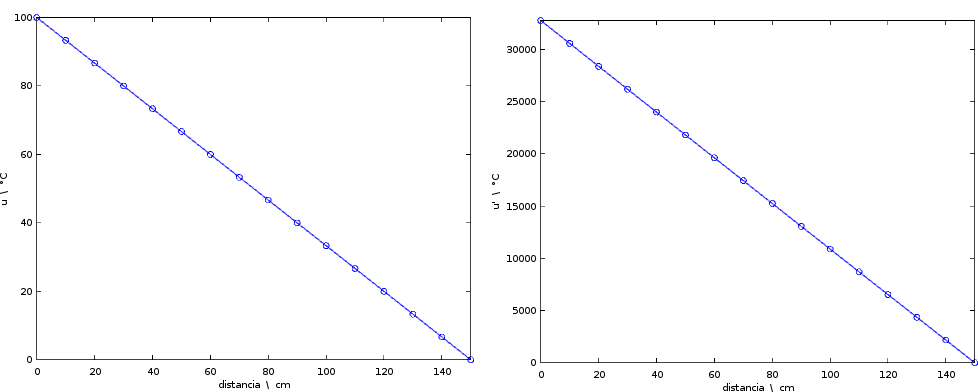
\includegraphics[scale=0.5]{u.png}
    \label{fig:secondlabel}
\end{minipage}

Perfil de temperaturas sobre la barra de metal en estado estcionario. Izquierda: escala original. Derecha: escala ampliada.






\end{document}